% Chapter Template

\chapter{Water-wave problem} % Main chapter title

\label{chapter3} % Change X to a consecutive number; for referencing this chapter elsewhere, use \ref{ChapterX}

%----------------------------------------------------------------------------------------
%	SECTION 1
%----------------------------------------------------------------------------------------

The theory of water waves has been a source of intriguing and difficult mathematical problems. Derived by Euler in 1757 (\cite{C2004}), the incompressible Euler equations with a free boundary, also known as the full water-wave problem, are widely regarded as the governing equations for water waves and have been the subject of extensive research. At first, the essential character of studying water waves was in bringing together equations of fluid mechanics, illustrating wave propagation, and highlighting the role of boundary conditions. However, during the last 60 years, the complexity of mathematical theories for water waves has exploded. The emergence of \textit{soliton} theory, itself conceived in the context of water waves, has transformed many mathematical aspects of nonlinear wave propagation. Today, the study of water waves is an important part of applied mathematics, serving as a diverse intersection in which many seemingly disparate parts of mathematics come together.

That water waves are a physical phenomenon has an added advantage: often, they may be analysed by direct observation. Indeed, mathematical results provide a description that can be tested whenever an expanse of water is at hand: a river, the ocean, or simply the household sink. In particular, such results may have wide-ranging implications in engineering and climate modelling. Conversely, numerical simulations by themselves have led to many advances in water waves. The complexity and variety of water-wave phenomena inform many applications but also invite other sciences to contribute, thereby making  the field suitable for multidisciplinary collaborations.

In this chapter, we delve into the water-wave problem. First, we explain the problem in greater detail and present the shallow water regime. Using asymptotic tools, we then describe and justify the derivation of the KdV model.

\section{Describing the water-wave problem}

Conservation of mass \eqref{S2:CoMass} and conservation of momentum \eqref{S2:CoMomentum} are the two core principles that provide the relevant equations of fluid dynamics. The resulting equations are 
\begin{align}
\frac{\partial \rho}{\partial t} + \nabla \cdot (\rho \V) &= 0, \label{S2:CoMass} \\
\rho\left[ v\frac{\partial \V}{\partial t} + (\V \cdot \nabla) \V\right] &= \textbf{F} - \nabla P + v_{\star} \Delta \V, \label{S2:CoMomentum}
\end{align}
where $\rho = \rho(\X, t)$ denotes the fluid mass density, $\V = \V(\X,t)$ is the fluid velocity, $P(\X, t)$ refers to pressure, $\textbf{F}(\X)$ is an external force, and $v_{\star}$ is the viscosity due to frictional forces. Derivations of \eqref{S2:CoMass} and \eqref{S2:CoMomentum} can be found in \cite[Chapter 1]{Johnson}. Assuming that the fluid is inviscid, incompressible, and irrotational, one can follow Section 5.1 of \cite{Ablowitz} to obtain the system
\begin{subequations} \label{S2:DimWholeLineProblem}
\begin{align}
\phi_{xx} + \phi_{zz} &= 0, &-h < z &< \eta(x,t), \label{S2:PDE}\\
\phi_{z} &= 0, &z &= -h, \label{S2:BBC}\\
\phi_t + g\eta + \frac{1}{2}(\phi_{x}^2 + \phi_{z}^2) &= 0, &z &= \eta(x,t), \label{S2:DBC}\\
\eta_t + \phi_{x}\eta_{x} &= \phi_{z}, &z &= \eta(x,t), \label{S2:KBC}
\end{align}
\end{subequations}
where $\phi(x,z, t)$ is a scalar field such that $\V = \nabla \phi$ and $\eta(x,t)$ is the surface elevation. In addition, $z$ is the vertical coordinate, $x$ is the horizontal direction, and $g$ is acceleration due to gravity. See Figure \ref{fig:waterwaveproblem} for a visual representation of the domain, which we denote $S = \RR \times (-h, \eta).$ In deriving \eqref{S2:DimWholeLineProblem}, the following assumptions are made:
\begin{itemize}
\item The problem has 1 horizontal dimension $x \in \RR.$
\item The fluid velocity $\V$ tends to equilibrium as $|x| \to \infty.$
\item The external force is the buoyancy due to gravity, i.e. $\textbf{F} = - \nabla (\rho_0 g z).$
\item The pressure vanishes on the surface, $P = 0$ at $z = \eta(x,t).$
\item The fluid density is constant, i.e. $\rho(\X,t) = \rho_0.$
\end{itemize}
As the problem is expressed in terms of $\phi,$ the scalar potential of velocity $\V,$ \eqref{S2:DimWholeLineProblem} is called the \textit{velocity potential} formulation of the water-wave problem.
\begin{figure}[h]
\captionsetup{width=\textwidth}
\centering
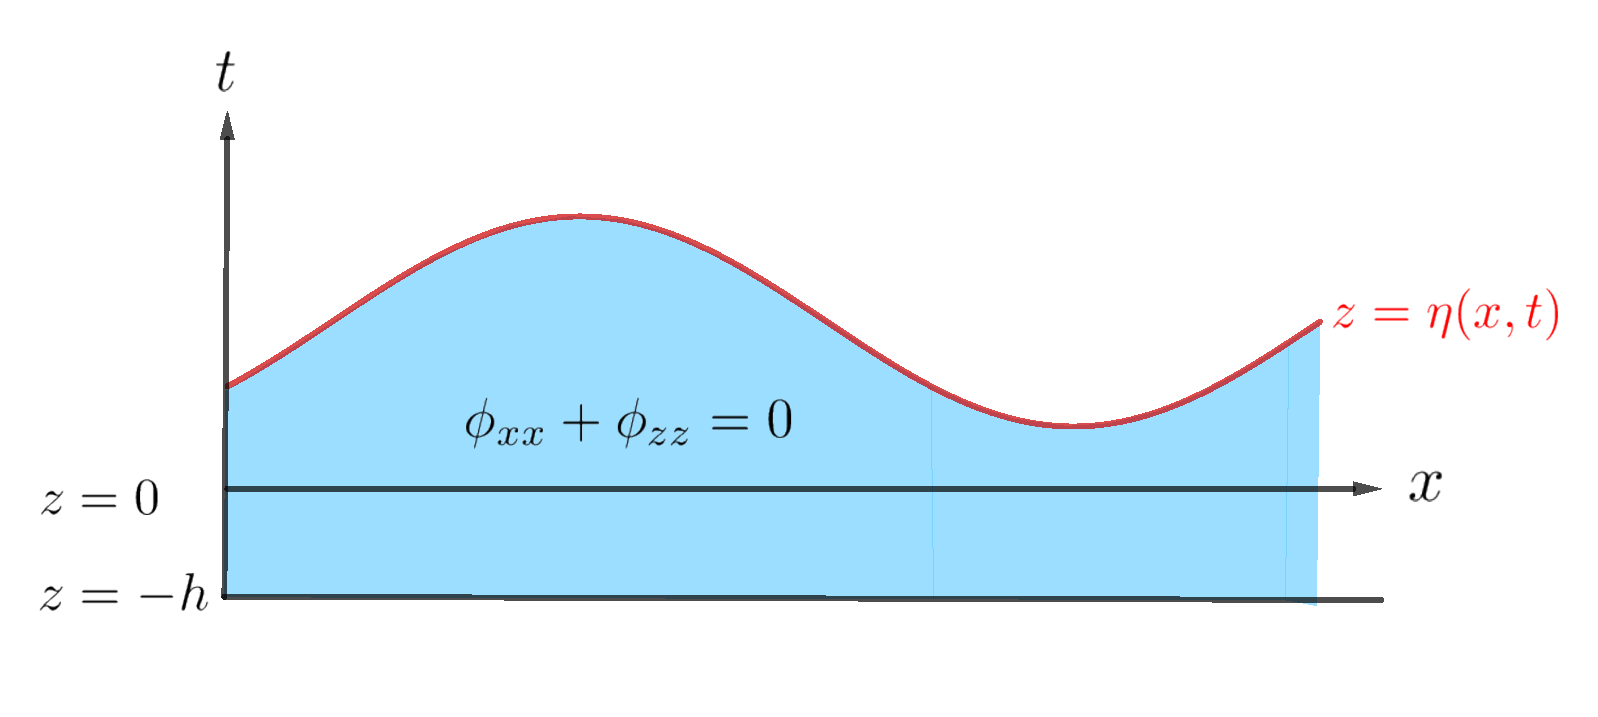
\includegraphics[width=\linewidth]{figures/waterwaveproblem.pdf}
\caption{Schematic for the domain of the water wave problem \eqref{S2:DimWholeLineProblem}.}
\label{fig:waterwaveproblem}
\end{figure}

We now describe the physical relevance of \eqref{S2:DimWholeLineProblem}, by explaining each equation:
\begin{itemize}
\item[\eqref{S2:PDE}:] Assuming that the fluid is irrotational means that the curl vanishes: $\nabla \times \V = 0.$ Thus, there is a scalar field $\phi$ such that $\nabla \phi = \V.$ Conservation of mass \eqref{S2:CoMass} then becomes $\Delta \phi = 0.$ In other words, the fluid inside the domain $S$ is incompressible and irrotational.
\item[\eqref{S2:BBC}:] This equation is an assumption that the bottom is a flat and impermeable surface, so that the fluid cannot escape through the bottom. Since $\phi_z$ is the vertical velocity, \eqref{S2:BBC} means that there is no flow through the bottom. We call \eqref{S2:BBC} \textit{the bottom condition}. 
\item[\eqref{S2:DBC}:] This equation is the conservation of momentum \eqref{S2:CoMomentum} applied at the surface $z = \eta(x,t).$ Since the conservation of momentum is a statement about the balance of external forces and fluid at the fluid's surface, this equation describes the dynamics of the velocity potential on the boundary. We call \eqref{S2:DBC} \textit{the dynamic boundary condition}.
\item[\eqref{S2:KBC}:] This equation represents the condition that $\eta$ is the surface of the fluid. In other words, the surface $z = \eta(x,t)$ is always composed of fluid particles that remain on the surface. We call \eqref{S2:KBC} \textit{the kinematic boundary condition}, since it describes the geometry and shape of the surface. The condition should be contrasted with the dynamic condition, which is about the interaction of forces acting at the surface. 
\end{itemize}

%Second, we explain some of the physical assumptions and considerations leading to the mathematical formulation of the problem. %While mostly following \cite[Chapter 1]{Lannes}, we also expound on some points and provide additional references. 
%Roughly speaking, the model is useful in applications to coastal oceanography, specifically in modelling tsunamis \cite{}.
%\begin{itemize}
%\item The fluid is assumed to be continuous. %We mainly deal with behaviour on scales that are large compared to the distance between molecules that comprise the fluid. 
%Physical quantities such as mass and velocity are spread continuously throughout the region; this is \textit{the continuity assumption}. %This is important to note, since water may have discontinuities in the form of air bubbles. Whenever this happens to a significant degree, e.g. when waves break, the problem \eqref{S2:DimWholeLineProblem} is no longer valid. A microscopic description of fluids is given by the Newton's laws and Boltzmann equation (see \cite{G2019} for a survey). 
%\item The fluid is assumed to be incompressible and inviscid. The fluid under study is pure water: its density does not change both in space and time, and it is mostly inviscid (see \cite[Appendix A2]{CK}). %One can extend the problem to work with compressible fluids. However, to account for viscosity, one needs to work with Navier-Stokes equations (see \cite[Section 1.3]{CM}. 
%\item The fluid is assumed to be irrotational. In applications considered here (e.g. tsunamis), rotational effects contribute little. %In reality, when the scales are much larger, rotational flows give rise to tornadoes, vortices and eddies. The situation is delicate when rotating effects are considered: the assumption $\V = \nabla \phi$ no longer holds, and the velocity formulation is replaced with the stream-function formulation. See \cite[p.32-35]{Lannes} for a detailed overview.
%\item The bottom is assumed to be flat. %In reality the bottom may differ drastically. Since the degree of bed rigidity, the porosity, and the roughness all influence the fluid to varying degrees, it is also more challenging to work with such bottoms. In addition, when working in the shallow water regime (as explained in the next section), it is necessary to make strong assumptions on the bottom to obtain correct asymptotics. As such, we choose to deal with the simplest case of a flat bottom. For a discussion of waves over more realistic seabeds, see \cite[Chapter 9]{DD}.
%\item We assume that the surface and the bottom of the domain can be parametrised as graphs. Neither the surface nor the bottom need to be functions; indeed, modelling overhanging waves is one such example. While this is true, assuming that the surface and the bottom are functions provides an easier setting to work in. 
%\item The fluid is contained in its domain. We assume that the fluid does not leak through its bottom, nor do the fluid particles leave the fluid surface. %These two conditions are given by \eqref{S2:BBC} and \eqref{S2:KBC}, respectively.
%%\item The fluid tends to equilibrium. This is a natural condition so long as one considers infinite domains such as the whole line. Note that any discussion of the rate of convergence relates to the \textit{stability} theory of water waves, and is not touched upon in this project.
%\item The water depth is assumed to be nonnegative. In other words, we have that $\eta - h > 0$ (see Figure \ref{fig:vanishingdepth}). %This is a major limitation, as it excludes vanishes shorelines. However, removing this assumption is an open problem. As the depth is vanishing, the size of computational domain becomes part of the solution $\phi.$ This issue leads to theoretical and numerical difficulties in describing the shoreline. There are some models that are extended to this case, though they are limited to one dimension and are not rigorously justified (see \cite{BCLMT2011}).
%\item The external force is conservative. This assumption follows naturally from conservation laws for water waves. %For our problem, relevant external forces are a \textit{body force}, which is the force due to an outside source and is identical for all fluid particles, and a \textit{local force}, which is the force exerted on a fluid particle by other particles. For our problem, gravity and pressure are pertinent body forces, and friction is the local force. Since the fluid is inviscid, no local force is present. See \cite[Chapter 4]{CK} for a detailed discussion.
%%\item The surface tension is negligible and the surface pressure is constant. In applications to coastal oceanography, the surface tension tends to be very small, which justifies the assumption (see \cite[Example 9.1, Chapter 9]{Lannes}). Since we expect no large weather variations, we can also assume that locally pressure is constant. Of course, surface tension is relevant when describing some smaller scale phenomena such as ripples. If one is to incorporate non-constant pressure and/or surface tension, the dynamic condition \eqref{S2:DBC} needs to be changed accordingly.
%%\item The system is two dimensional: there is one spatial dimension $x$ and one vertical dimension $z.$ By ignoring the remaining dimension $y,$ we assume that the fluid is moving in $x$ direction only. In other words, we consider the special case of \textit{no transverse waves}.  Incorporating weak transverse variation leads to a generalisation of the KdV equation, the Kadomtsev-Petviashvili equation:
%%\begin{equation}\label{S2:KP}
%%\partial_x(u_t + 6uu_x + u_{xxx}) + 3 \rho u_{yy} = 0.
%%\end{equation}
%%In \eqref{S2:KP}, if $\rho = 1,$ then water waves with small surface tension are modelled, and if $\rho = -1,$ then water waves with large surface tension are modelled.
%\end{itemize}
\rmk{While the wave motion is expected to be initiated in some fashion, we are mainly interested in evolution of wave motion. As such, initial conditions are not explicitly discussed.}

%\begin{figure}[h]
%\captionsetup{width=\textwidth}
%\centering
%    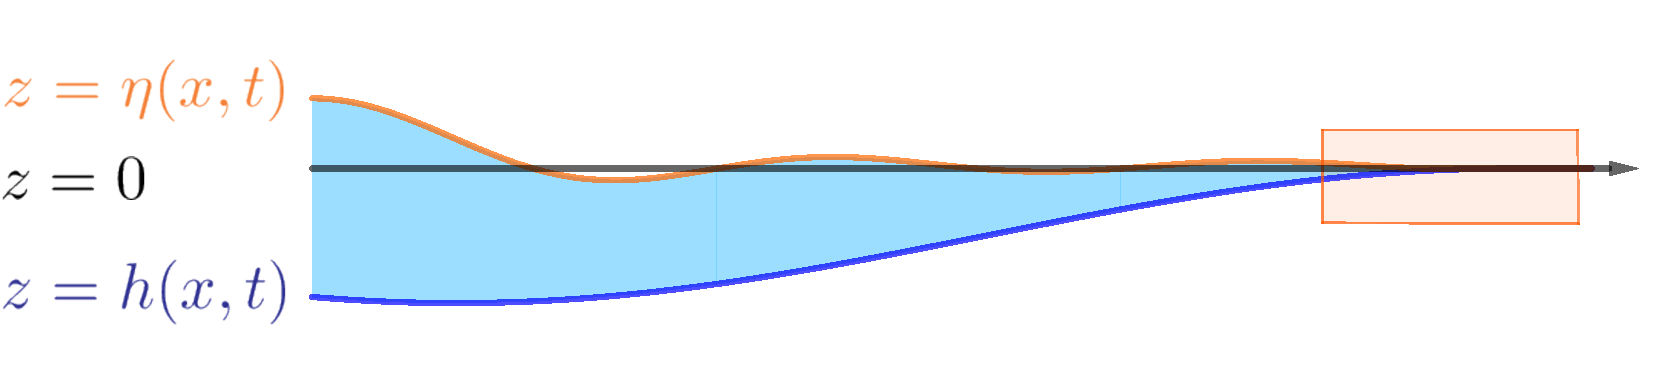
\includegraphics[width=\linewidth]{figures/vanishingdepth2.pdf}
%  \caption{The region in orange is the zone of vanishing water depth. In this region, the domain becomes part of the solution, which complicates the problem. Therefore, the problem \eqref{S2:DimWholeLineProblem} is valid in the zone to the left of the orange region.}
%  \label{fig:vanishingdepth}
%\end{figure}

\section{Shallow water regime} 
For now, \eqref{S2:DimWholeLineProblem} admits numerous types of water waves: short waves, long waves, intermediate waves. This is because we have yet to specify how wavelength relates to the water depth. Thus, we first examine the \textit{dispersion relation}, which describes the relation between wave velocity and wavelength. This will allow us to focus on the shallow water regime.

We consider small-amplitude waves, or equivalently, we assume that $|\eta| \ll 1$ and $\Vert \nabla \phi \Vert \ll 1.$ The dispersion relation is obtained by linearising the problem \eqref{S2:DimWholeLineProblem} around $z=0.$ More concretely, let $\phi_s(x,z,t) = \tilde{\phi}(k,z,t) \exp(ikx),$ and $\eta_s(x,t) = \tilde{\eta}(k,t)\exp(ikx);$ we think of $\phi_s$ and $\eta_s$ as special form solutions $\phi$ and $\eta.$ We then may follow Section 5.2 of \cite{Ablowitz}, to obtain the following ODE:
\[ 
\frac{\partial^2 \tilde{\eta}}{\partial t^2} + g k \tanh(k h) \tilde{\eta} = 0.
\]
Assuming that $\tilde{\eta}(k,t) = \tilde{\eta}(k, 0) \exp(-i \omega t),$ the above equation yields the dispersion relation $\omega^2 = g k \tanh(k h).$ Here, $\omega$ is a frequency, $k$ is a wave number, and $g$ is gravity. 

With this in mind, we focus on the shallow water regime, characterised by small-amplitude waves that have long wavelength relative to the water depth. For shallow water, the wavelength $\dfrac{2 \pi}k{}$ is much bigger than the depth $h,$ so $kh \ll 1.$ Expansion of $\tanh(kh)$ in $kh$ allows to rewrite the dispersion relation as
\[ \omega^2 = gk(kh - \frac{(kh)^3}{3} + \mathcal{O}((kh)^5))  \simeq ghk^2. \]
Thus, small-amplitude waves in shallow water have frequency $ \omega = \pm \sqrt{gh}|k|,$ or equivalently, velocity $c_0 = \sqrt{gh}.$ Now, using the dispersion relation, we can \textit{rescale} the problem \eqref{S2:DimWholeLineProblem} to model shallow water waves with velocity $c_0 = \sqrt{gh}.$ In nature, tsunamis and tidal waves are examples of this regime. 

In addition, the problem \eqref{S2:DimWholeLineProblem} does not specify the physical dimensions. Since dimensions of the problem are directly related to the units of variables such as wavelength, time, or height, it can be difficult to decide which terms are negligible when performing asymptotic reductions. The process of \textit{non-dimensionalisation} removes the physical dimensions, allowing us to work with "pure" numbers. Letting primes denote the dimensionless variables, we introduce
\begin{equation}\label{S2:NDvar}
z = hz' \qquad x = \lambda x' \qquad t = \frac{\lambda}{c_0}t' \qquad \eta = a \eta' \qquad \phi = \frac{\lambda g a}{c_0} \phi',
\end{equation}
where $c_0 = \sqrt{gh}$ is the shallow water speed, $\lambda$ is the wavelength and $a$ is the maximum amplitude of initial data. See Sections 1.3.2-1.3.3 of \cite{Lannes} for a detailed discussion of \eqref{S2:NDvar}. 

We define parameters $\epsilon = \dfrac{a}{h}, \mu = \dfrac{h}{\lambda}.$ Physically, $\epsilon$ is an amplitude of a wave relative to depth, while $\mu$ is a ratio of depth to a typical wavelength. Alternatively, we understand that $\epsilon$ measures nonlinearity and $\mu$ measures dispersion. 
%Transforming \eqref{S2:DimWholeLineProblem} via chain rule and dropping the primed notation yields 
%\begin{subequations}\label{S2:WLPND1}
%\begin{align}
%\mu^2 \phi_{xx} + \phi_{zz} &= 0, &-1 < z &< \varepsilon\eta, \label{S2:PDEND1} \\
%\phi_z &= 0, &z &= -1, \label{S2:BC1ND1} \\ 
%\phi_{t} + \frac{\varepsilon}{2} \left(\phi_{x}^2 + \frac{1}{\mu^2}\phi_{z}^2\right) + \eta &= 0, &z &= \varepsilon\eta(x,t), \label{S2:BC2ND1} \\
%\mu^2 \left[\eta_{t} + \varepsilon \phi_{x} \eta_{x}\right] &= \phi_{z}, &z &= \varepsilon\eta(x,t). \label{S2:BC3ND1} 
%\end{align}
%\end{subequations}
%The problem \eqref{S2:WLPND1} is a "normalised" problem that models shallow water waves.

Note that we have yet to make any assumptions about $\epsilon$ and $\mu,$ nor is any relationship between the two parameters prescribed. We make the following assumptions:
\begin{itemize}
\item Assume $\mu \ll 1.$ Recall that $\mu$ is a ratio of depth to wavelength, and in shallow water regime, we expect that depth is much smaller compared to wavelength.
\item To obtain interesting approximate equations, we should balance the parameters by connecting them to each other. This is \textit{the principle of maximal balance} (see \cite{Kruskal1963}). We choose $\varepsilon = \mu^2,$ which reflects the balance of weak nonlinearity and weak dispersion.
\item From the maximal balance principle, we have $\epsilon \ll 1.$ Physically, we consider water waves whose amplitude is small relative to depth.
\end{itemize}
Transforming \eqref{S2:DimWholeLineProblem} via chain rule and dropping the primed notation yields 
\begin{subequations}\label{S2:WLPND2}
\begin{align}
\label{S2:PDEND2}  \varepsilon\phi_{xx} + \phi_{zz} &= 0, &-1 <z &< \varepsilon\eta, \\
\label{S2:BC1ND2} \phi_z &= 0, &z &= -1,  \\ 
\label{S2:BC2ND2} \phi_{t} + \frac{1}{2} \left(\varepsilon\phi_{x}^2 + \phi_{z}^2\right) + \eta &= 0, &z &= \varepsilon\eta(x,t),\\
\label{S2:BC3ND2} \varepsilon\left[\eta_{t} + \varepsilon \phi_{x} \eta_{x}\right] &= \phi_{z}, &z &= \varepsilon\eta(x,t).
\end{align}
\end{subequations}
The problem \eqref{S2:WLPND2} is a "normalised" problem that models small-amplitude shallow water waves.

\rmk{
Note that there is no reason not to balance in other ways, say $\varepsilon = \sqrt{\mu}.$ There are many options: some lead to interesting equations, while others do not. Indeed, it is this assumption in the procedure that determines the relevance of the model derived below.}

\section{Deriving the KdV model}
The presence of $\epsilon$ in \eqref{S2:WLPND2} indicates that we can further simplify the problem using ideas developed in Chapter 2. Expanding $\phi(x,z,t) = \phi_0(x,z,t) + \epsilon \phi_1(x,z,t) + \mathcal{O}(\epsilon^2)$ and substituting the series into \eqref{S2:PDEND2} and \eqref{S2:BC1ND2} yields
\begin{equation}\label{S2:PS0}
\phi = A - \frac{\epsilon}{2} A_{xx}(z+1)^2 + \frac{\epsilon^2}{4!} A_{xxxx} (z+1)^4 + \mathcal{O}(\epsilon^3)
\end{equation}
valid in $-1<z<\epsilon \eta,$ where $\phi_0 = A(x,t).$ Substituting \eqref{S2:PS0} into \eqref{S2:BC2ND2} and \eqref{S2:BC3ND2}, along with appropriate manipulations, gives
\begin{equation}\label{S2:PS1}
A_{tt} - A_{xx} = \epsilon\left( \frac{A_{xxxx}}{3} - 2A_x A_{xt} - A_{xx}A_t\right),
\end{equation}
valid up to $\mathcal{O}(\epsilon).$ Obtaining \eqref{S2:PS1} is an especially lengthy calculation, since the dynamic and kinematic conditions must be expanded carefully. 

Now, we sketch out the derivation of the KdV model. Expanding $A = A_0 + \epsilon A_1 + \mathcal{O}(\epsilon^2)$ and substituting this expansion into \eqref{S2:PS1}, we have 
\begin{equation}\label{S2:W1}
\mathcal{O}(\epsilon^0): \quad A_{0tt} - A_{0xx} = 0.
\end{equation} 
This is the wave equation, whose general solution is $A_0 = F(x-t) + G(x+t),$ for some functions $F,G.$

We would like to determine $F,G.$ First, we observe that in parallel to the Duffing oscillator, \eqref{S2:PS1} contains secularities in $t$ when solving the next order euqation. %, or one could solve \eqref{S2:PS1} numerically and see that the solution is unbounded in time.
This can partly be shown via the dispersion relation and therefore an introduction of multiple time scales: $\tau_0 = t, \tau_1 = \epsilon t.$ We also let $\xi = x- \tau_0$ and $\zeta = x + \tau_0,$ so that $A_0 =  F(\xi, \tau_1) + G(\zeta, \tau_1).$ Via appropriate calculations, from \eqref{S2:PS1} one obtains 
\begin{align}
2F_{\tau_1} + \frac{1}{3}F_{\xi\xi\xi} + 3 F F_\xi &= 0, \label{S2:KdV1} \\
2G_{\tau_1} - \frac{1}{3}G_{\zeta\zeta\zeta} -  3 G G_\zeta &= 0. \label{S2:KdV2}
\end{align}
Hence, we obtain two KdV equations, \eqref{S2:KdV1} and \eqref{S2:KdV2}, which determine the dependence of $F, G$ on $\tau_1.$ Solving the KdV equations via initial conditions, we determine $\phi_0 = A_0,$ and therefore $\phi$ in the leading order.

The wave and KdV equations are well-known PDEs. The wave equation arises as a model in numerous fields of physics, such as electrodynamics, plasma physics, and general relativity. The KdV equation appears whenever long waves propagate over dispersive media, be it in the fields of fluid mechanics, nonlinear optics, or Bose-Einstein condensates. Because of how they occur independently of applications, the two equations have been studied extensively. Furthermore, the KdV equation is special: despite being nonlinear, it can be solved exactly in certain domains, using advanced techniques such as the inverse scattering transform (see Chapter 9 of \cite{Ablowitz}).

In conclusion, the leading order solution of the water wave problem for small-amplitude, shallow water waves is described by the wave equation \eqref{S2:W1} and two KdV equations \eqref{S2:KdV1}, \eqref{S2:KdV2}. This is the result we seek to obtain on the whole line using a different formulation of the problem, as well as a new extension to the half-line.

\section{Are asymptotic methods reliable?}
Given the emphasis on asymptotic and perturbative methods, one is interested whether these methods provide "reliable" solutions. Formally, how can we justify that solutions of asymptotic equations converge to solutions of the original problem? In the context of the water-wave problem \eqref{S2:DimWholeLineProblem}, is the KdV model, provided by the shallow water approximation, "reasonable"? Of course, in asking these questions, one needs to specify the meaning of ``reliable" and ``reasonable". Following \cite{Lannes}, the validity of the KdV model can be understood from the following questions:
\begin{enumerate}
\item Do the solutions of \eqref{S2:DimWholeLineProblem} exist on the required time scale?
\item Do the solutions of the KdV model exist on the same time scale?
\item Are the asymptotic solutions close to the actual solutions with the corresponding initial data? If so, how close?
\end{enumerate}
If the answer to all three questions is positive, then the asymptotic model is \textit{fully justified}. Indeed, the KdV model is fully justified (see \cite[p. 297-298]{Lannes}). The detailed proofs require advanced mathematics such as working in Sobolev spaces and applying Poincaré and Gagliardo-Nirenberg inequalities. Since the rigorous mathematical justification of the KdV model is beyond the scope of the project, we choose not to discuss this topic here, and refer the reader to Chapter 7 and Appendix C of \cite{Lannes} for the details.